\documentclass{beamer}
\usetheme{metropolis}
\usepackage{listings}
%Information to be included in the title page:
\title{Progetto e integrazione del supporto ad Alibaba Cloud su Noovolari Leapp}
\author{Andrea Pusineri}
\institute{Università di Pavia}
\date{2020/2021}

\lstdefinestyle{customgo}{
  language=Go,
  breaklines=true,
  basicstyle=\footnotesize\ttfamily,
  xleftmargin=\parindent,
  numbers=left,
  stepnumber=1,
  showstringspaces=false,
  tabsize=2,
  escapeinside=||
}

%%%%%%%%%%%%%%%%%%%% Scripts %%%%%%%%%%%%%%%%%%%
% Stoppa il count nei listing
\let\origthelstnumber\thelstnumber
\makeatletter
\newcommand*\Suppressnumber{%
  \lst@AddToHook{OnNewLine}{%
    \let\thelstnumber\relax%
     \advance\c@lstnumber-\@ne\relax%
    }%
}

% Riprende il count nei listing a partire da un numero specificato
\newcommand*\Reactivatenumber[1]{%
  \setcounter{lstnumber}{\numexpr#1-1\relax}
  \lst@AddToHook{OnNewLine}{%
   \let\thelstnumber\origthelstnumber%
   \refstepcounter{lstnumber}
  }%
}

\begin{document}
%%%%%%%%%%%%%%% Title Page %%%%%%%%%%%%%%%
\frame{\titlepage}
%%%%%%%%%%%%%%% Table of Contents %%%%%%%%%%%%%%%
%\begin{frame}
%\frametitle{Contenuti}
%\tableofcontents
%\end{frame}
%%%%%%%%%%%%%%% Introduzione %%%%%%%%%%%%%%%
\section{Introduzione}
\begin{frame}
 \frametitle{Introduzione}
  \begin{itemize}
  \item<1-> \textbf{beSharp} è un’azienda specializzata nell’implementazione e gestione di infrastrutture e servizi Cloud su AWS.
  \item<2-> \textbf{Noovolari} è una sezione di beSharp che si concentra sulla ricerca e sviluppo.
  \item<3-> \textbf{Leapp} è uno strumento che semplifica e rende più sicura la gestione delle credenziali di accesso al Cloud.
  \item<4-> \textbf{Alibaba Cloud}, sussidiaria dell’Alibaba Group, è il più grosso fornitore di cloud computing cinese.
  \item<5-> \textbf{Progetto} dell'integrazione del supporto ad Alibaba Cloud, in linea con i metodi di autenticazione esistenti.
 \end{itemize}
\end{frame}

\begin{frame}
 \frametitle{Introduzione}
  \begin{figure}
   \centering
   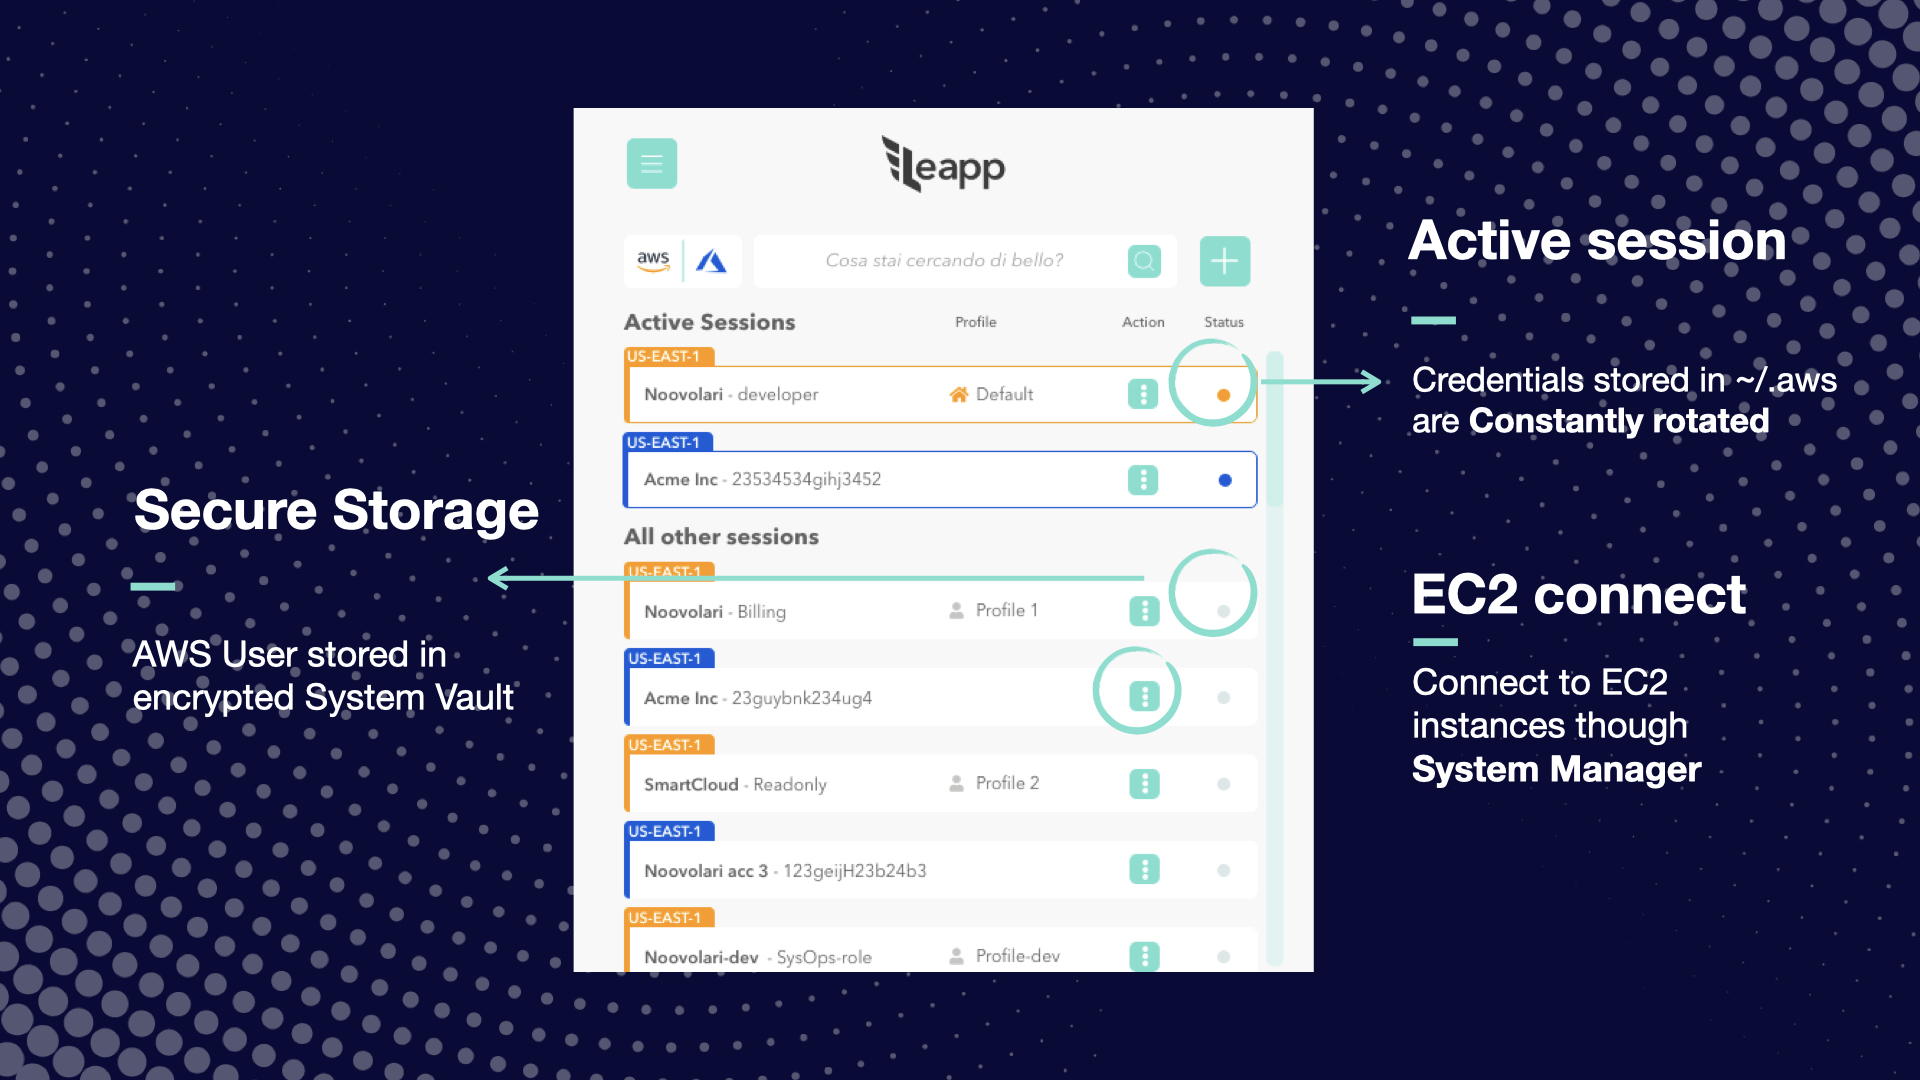
\includegraphics[width=1\textwidth]{Risorse/leapp_presentazione.jpeg}
  \end{figure}
\end{frame}
%%%%%%%%%%%%%%% Cloud Computing %%%%%%%%%%%%%%%
%\section{Cloud Computing}
%\begin{frame}
%\frametitle{Cloud Computing}
 %Il Cloud Computing è un modello che consente l’utilizzo on-demand di un poolcondiviso di risorse computazionali programmabili che possono essere rese disponibili velocemente e in modo automatizzato, richiedendo un’interazione minima da parte delfornitore.
%\end{frame}
%
%\begin{frame}
% \frametitle{Cloud Computing - Caratteristiche}
% \begin{itemize}
%  \item \textbf{On-demand self-service}
%  \item \textbf{Broad network access}
%  \item \textbf{Resource pooling}
%  \item \textbf{Rapid elasticity}
%  \item \textbf{Measured service}
% \end{itemize}
%
%\end{frame}
%%%%%%%%%%%%%%% Leapp %%%%%%%%%%%%%%%
\section{Leapp}
\begin{frame}
 \frametitle{Leapp}
 Leapp è costituita da due componenti principali:
 \begin{itemize}
  \item<2-> una \textbf{GUI} sviluppata in Typescript mediante il framework Electron.
  \item<3-> un \textbf{demone}, scritto in Go, eseguito in background, che svolge automaticamente diverse operazioni di gestione e manutenzione delle credenziali.
 \end{itemize}
\end{frame}

\begin{frame}
 \frametitle{Leapp - Clean Architecture}
 Architettura software che mediante la divisione in livelli punta a produrre un sistema:
 \begin{itemize}
  \item Indipendente dai framework
  \item Testabile
  \item Indipendente dalla UI
  \item Indipendente dal database
  \item Indipendente da fattori esterni
 \end{itemize}
\end{frame}

\begin{frame}
 \frametitle{Leapp - Clean Architecture}
 \begin{figure}
   \centering
   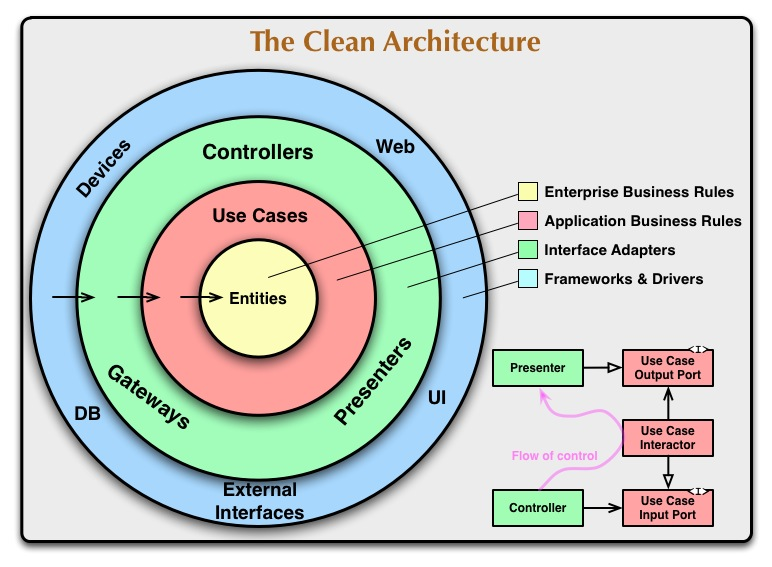
\includegraphics[width=1\textwidth]{Risorse/CleanArchitecture.jpg}
  \end{figure}
\end{frame}

\begin{frame}[fragile]
 \frametitle{Leapp - Clean Architecture - Dependency rule}
 \textbf{Dependency rule}: le dipendenze possono puntare solo verso l’interno, nulla dei livelli più interni può assumere nulla sui più esterni.
 \pause

 \textbf{Dependency injection}: l’idea che i componenti del sistema (strutture in Go) debbano ricevere le dipendenze alla creazione
\end{frame}

\begin{frame}[fragile]
 \frametitle{Leapp - Clean Architecture - Dependency rule}
 \begin{lstlisting}[style=customgo, caption=esempio di Dependency Injection, captionpos=b]
 type Server struct {
     config *Config
 }

 func New() *Server {
     return &Server{
         config: buildConfig(),
     }
 }
 \end{lstlisting}
\end{frame}


%%%%%%%%%%%%%%% Esperienza di tirocinio %%%%%%%%%%%%%%%
\section{Esperienza di tirocinio}
\begin{frame}
 \frametitle{Esperienza di tirocinio - Alibaba RAM}
 Alibaba Cloud \textbf{Resource Access Management} (RAM) è un servizio che permette di gestire le identità di accesso all'interno di un account Alibaba Cloud.
 \pause

 \begin{itemize}
  \item \textbf{Utenti}: identità composte da un ID e delle credenziali.
  \pause
  \item \textbf{Ruoli}: identità virtuali a cui è associato un insieme di permessi definiti tramite policies.
 \end{itemize}
\end{frame}

\begin{frame}
 \frametitle{Esperienza di tirocinio - Alibaba RAM - Autenticazione}
 Alibaba Cloud permette l'autenticazione in diversi modi, i più importanti ai fini del progetto sono:
 \pause

 \begin{itemize}
  \item \textbf{AccessKey pair}: una coppia di chiavi alfanumeriche, un \textit{AccessKey ID} e un \textit{AccessKey Secret}.
  \pause
  \item \textbf{StsToken}: un stringa che permette l’assunzione di un ruolo per una limitata finestra di tempo.
  \pause
  \item \textbf{Single Sign-On}: utilizza il protocollo SAML2.0 per l’autenticazione tramite federazione.
 \end{itemize}
\end{frame}

\begin{frame}
 \frametitle{Esperienza di tirocinio - Struttura progetto}
 \begin{figure}
   \centering
   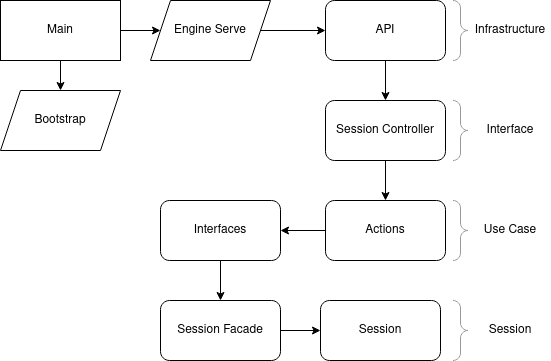
\includegraphics[width=0.9\textwidth]{Risorse/PianoForge.png}
  \end{figure}
\end{frame}

\begin{frame}[fragile]
 \frametitle{Esperienza di tirocinio - Sviluppo - RAM User Access}
 \centering
 Esempio: creazione di una nuova session\\
 \textbf{Infrastruttura}\\
 \begin{lstlisting}[style=customgo, caption=engine.go (righe 53-92), captionpos=b, firstnumber=53]
func initializeRoutes(ginEngine *gin.Engine) {
  v1 := ginEngine.Group("/api/v1") { |\Suppressnumber|
...|\Reactivatenumber{85}|
    v1.GET("/alibaba/ram-user-sessions/:id", controller.GetAlibabaRamUserSessionController)
    v1.POST("/alibaba/ram-user-sessions/", controller.CreateAlibabaRamUserSessionController)|\Suppressnumber|
...|\Reactivatenumber{91}|
  }
}
 \end{lstlisting}
\end{frame}

\begin{frame}[fragile]
 \frametitle{Esperienza di tirocinio - Sviluppo - RAM User Access}
 \centering
 \textbf{Interfaccia}\\
 \begin{lstlisting}[style=customgo, caption=alibaba\_ram\_user\_session\_actions.go (righe 18-40), captionpos=b, firstnumber=18]
func (actions *AlibabaRamUserSessionActions) Create(alias string, alibabaAccessKeyId string, alibabaSecretAccessKey string, regionName string, profileName string) error { |\Suppressnumber|
...|\Reactivatenumber{30}|
	alibabaRamUserAccount := session.AlibabaRamUserAccount{ |\Suppressnumber|
...|\Reactivatenumber{33}|
	}

	sess := session.AlibabaRamUserSession{ |\Suppressnumber|
...|\Reactivatenumber{39}|
      Account: &alibabaRamUserAccount,
	}
 \end{lstlisting}
\end{frame}

\begin{frame}[fragile]
 \frametitle{Esperienza di tirocinio - Sviluppo - RAM User Access}
 \centering
 \textbf{Interfaccia}\\
 \begin{lstlisting}[style=customgo, caption=alibaba\_ram\_user\_session\_actions.go (righe 42-58), captionpos=b, firstnumber=42]
	err = actions.AlibabaRamUserSessionsFacade.AddSession(sess)
	if err != nil {
		return err
	} |\Suppressnumber|
...|\Reactivatenumber{52}|
	err = actions.Keychain.SetSecret(alibabaSecretAccessKey, sess.Id+constant.PlainAlibabaSecretAccessKeySuffix) |\Suppressnumber|
...|\Reactivatenumber{58}|
}
 \end{lstlisting}
\end{frame}

\begin{frame}[fragile]
 \frametitle{Esperienza di tirocinio - Sviluppo - RAM User Access}
 \centering
 \textbf{Use Case}\\
 \begin{lstlisting}[style=customgo, caption=alibaba\_ram\_user\_session\_facade.go (righe 64-92), captionpos=b, firstnumber=64]
func (fac *AlibabaRamUserSessionsFacade) AddSession(alibabaRamUserSession AlibabaRamUserSession) error {
	alibabaRamUserSessionsLock.Lock()
	defer alibabaRamUserSessionsLock.Unlock()

	oldAlibabaRamUserSessions := fac.GetSessions()
	newAlibabaRamUserSessions := make([]AlibabaRamUserSession, 0) |\Suppressnumber|
...|\Reactivatenumber{90}|
	newAlibabaRamUserSessions = append(newAlibabaRamUserSessions, alibabaRamUserSession)

	err := fac.updateState(newAlibabaRamUserSessions)
 \end{lstlisting}
\end{frame}

\begin{frame}[fragile]
 \frametitle{Esperienza di tirocinio - Sviluppo - RAM User Access}
 \centering
 \textbf{Session}\\
 \begin{lstlisting}[style=customgo, caption=alibaba\_ram\_user\_session.go (righe 9-19), captionpos=b, firstnumber=9]
type AlibabaRamUserSession struct {
	Id      string
	Alias   string
	Status  Status
	Account *AlibabaRamUserAccount
}

type AlibabaRamUserAccount struct {
	Region         string
	NamedProfileId string
}
 \end{lstlisting}
\end{frame}

\begin{frame}[fragile]
 \frametitle{Esperienza di tirocinio - Sviluppo - RAM Role Federated}
 \centering
 \textbf{Autenticazione tramite SAML}\\
 \begin{lstlisting}[style=customgo, caption=alibaba\_ram\_role\_federated\_session\_actions.go (righe 20-28), captionpos=b, firstnumber=20]
func SAMLAuth(region string, idpArn string, roleArn string, assertion string) (key string, secret string, token string, err error) {
	client, _ := sts.NewClientWithAccessKey(region, "", "")

	request := sts.CreateAssumeRoleWithSAMLRequest()
	request.Scheme = "https"
	request.SAMLProviderArn = idpArn
	request.RoleArn = roleArn
	request.SAMLAssertion = assertion
	response, err := client.AssumeRoleWithSAML(request)
 \end{lstlisting}
\end{frame}

\begin{frame}[fragile]
 \frametitle{Esperienza di tirocinio - Sviluppo - RAM Role Chained}
 \centering
 \textbf{Concatenzaizone di ruoli}\\
 \begin{lstlisting}[style=customgo, caption=alibaba\_ram\_role\_chained\_session.go (righe 9-29), captionpos=b, firstnumber=9]
type AlibabaRamRoleChainedSession struct {
	Id            string
	Status        Status
	StartTime     string
	ParentId      string
	ParentType    string
	Account       *AlibabaRamRoleChainedAccount
	Profile       string
}

type AlibabaRamRoleChainedAccount struct {
	AccountNumber string
	Name          string
	Role          *AlibabaRamRole
	Region        string
}
 \end{lstlisting}
\end{frame}

\begin{frame}[fragile]
 \frametitle{Esperienza di tirocinio - Sviluppo - RAM Role Chained}
 \centering
 \textbf{Parent Session}\\
 \begin{lstlisting}[style=customgo, caption=parent\_interface.go (righe 3-6), captionpos=b, firstnumber=3]
type ParentSession interface {
	GetId() string
	GetTypeString() string
}
 \end{lstlisting}
\end{frame}

\begin{frame}
 \frametitle{}
 \centering
 \textbf{Grazie per l'attenzione}\\
\end{frame}

\end{document}
